\documentclass[11pt]{article}
\author{Tarang Srivastava}
\usepackage{amsmath, amsthm}
\usepackage{graphicx}
\usepackage{multicol}
\usepackage{esdiff}
\usepackage[margin=.25in]{geometry}
\geometry{letterpaper,textwidth=7.3in,hmarginratio=1:1,	textheight=9in,vmarginratio=1:1,heightrounded}
\newcommand{\makechaptertitle}[1]{
\begin{center}
	\begin{large}
		DECA End of Chapter #1 Quiz
	\end{large}
	\begin{small}
		\\by Tarang Srivastava
	\end{small}
\end{center}
}
\theoremstyle{definition}
\renewcommand{\theenumi}{\alph{enumi}}
\newtheorem{q}{}
\begin{document}
	\begin{multicols*}{2}
		\makechaptertitle{6}
		You are allowed to use a Laplace transform table to solve these problems. (Page 321)
		\begin{q}
			Find the solution of the differential equation using the Laplace Transform\[ y'' + y = \sin 2t \] satisfying the initial condition \[ y(0) = 2, \indent y'(0) = 1 \]
		\end{q}
		\begin{q}
			Find the inverse transform of 
			\[ F(s) = \dfrac{1-e^{-2s}}{s^2} \]
		\end{q}
		\begin{q}
			Find the inverse transform of \[ H(s) = \dfrac{a}{s^2(s^2+a^2)} \]
		\end{q}
		\begin{q}
			Consider a rope with mass M and of length L. Solve for the equation of the displacement of the rope with respect to time \\ \\
			\begin{center}
				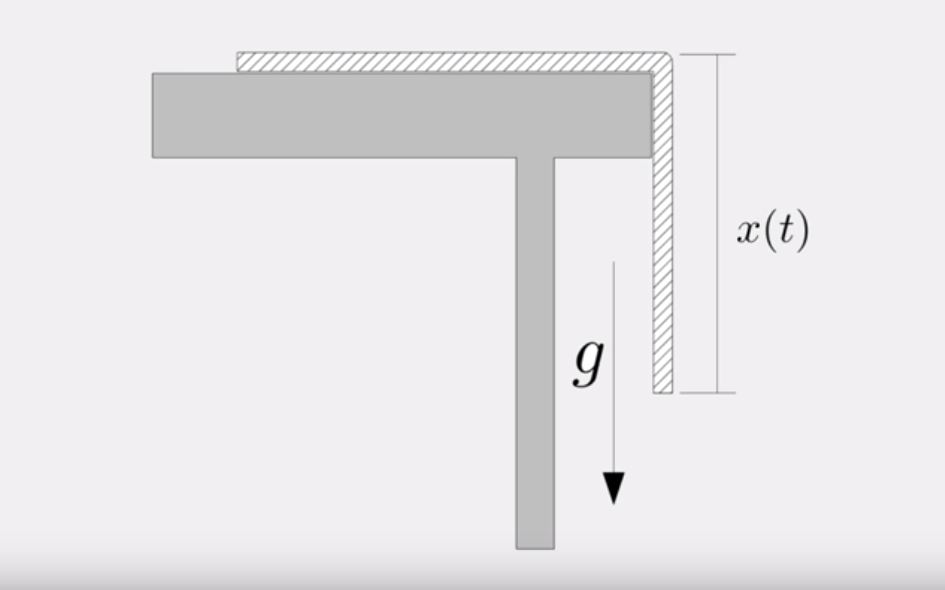
\includegraphics[width=8cm]{ropemass}
			\end{center}

		\end{q}
	
		\begin{q}
			\textbf{The Tautochrone} - the curve down which a particle will slide freely under gravity alone, reaching the bottom in time regardless of its starting point on the curve. \\
			A figure of the curve is shown on the side. The starting point is $ P(a,b) $ and the end point is the origin. \\ 
			\begin{center}
				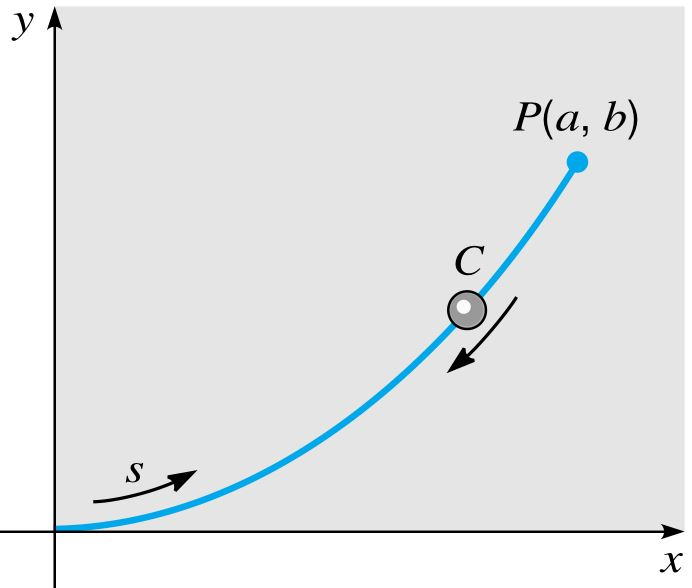
\includegraphics[width=8cm]{taut} 
			\end{center}
			\begin{enumerate}
				\item Given that the Arc length $ s $ is measured from the origin and $ f(y) $ gives the rate of change of $ s $ with respect to $ y $. 
			\[ f(y) = \dfrac{ds}{dy} = \left[1 + \left( \dfrac{dx}{dy} \right)^2 \right]^{1/2} \]
				\item Using conservation of energy the time $ T(b) $ required for a particle to slide from $ P $ to the origin is (Show this step!!)
				\[ T(b) = \dfrac{1}{\sqrt{2g}} \int_{0}^{b}\dfrac{f(y)}{\sqrt{b-y}} dy\]
			\item By the property of a Tautochrone the value of $ T(b) = T_0 $ is a constant for each $ b $. Taking the Laplace transform show that 
			\[ F(s) = \sqrt{\dfrac{2g}{\pi}} \dfrac{T_0}{\sqrt{s}} \] 
			\item Then show that 
			\[ f(y) = \dfrac{\sqrt{2g}}{\pi} \dfrac{T_0}{\sqrt{y}}\] 
			\item Using the previous answers show 
			\[ \dfrac{dx}{dy} = \sqrt{\dfrac{2 \alpha - y}{y}} \]
			where $ \alpha = gT_0^2/\pi^2 $ 
			\item Use the substitution $ y = 2 \alpha \sin ^2 (\theta / 2)$ and show 
			\[ x = \alpha (\theta + \sin \theta) \] \[ y = \alpha (1-\cos \theta)\] 
			Which is a parametric equation of a cycloid, the solution to the problem
			\end{enumerate}
			
			
		\end{q}
	\end{multicols*}
\end{document}
